\documentclass{beamer}

%\setbeameroption{show notes}
\setbeamercovered{transparent} 

\usepackage[english]{babel}

\usepackage{fontspec}
% \setmainfont{SemiSerif}
% \setmonofont{Mono}
% \setsansfont{Sans}

\usepackage{xcolor}
\usepackage{graphicx}
\usepackage{tikz-cd}
\usetikzlibrary{shapes,fit}
\beamertemplatenavigationsymbolsempty

\def\ci{\perp\!\!\!\perp}

\usepackage{listings}
\lstset{language=Python}

\usepackage{biblatex}
\bibliography{bibliography.bib}
\bibliography{simuling.bib}

\usefonttheme[onlymath]{serif}
\usetheme{Warsaw}

\title{Models and databases for Eastern Indonesia}
\author{Gereon Kaiping}
\institute{Out of Asia project, Phylogeography (GIScience)}
\date{2019-10-25}

\begin{document}

\begin{frame}[plain]
  \titlepage
\end{frame}
\begin{frame}
  \tableofcontents
\end{frame}
\section{Timor-Alor-Pantar languages}
\begin{frame}{Timor-Alor-Pantar languages}
  W-most “Papuan” language family in contact with Austronesian

  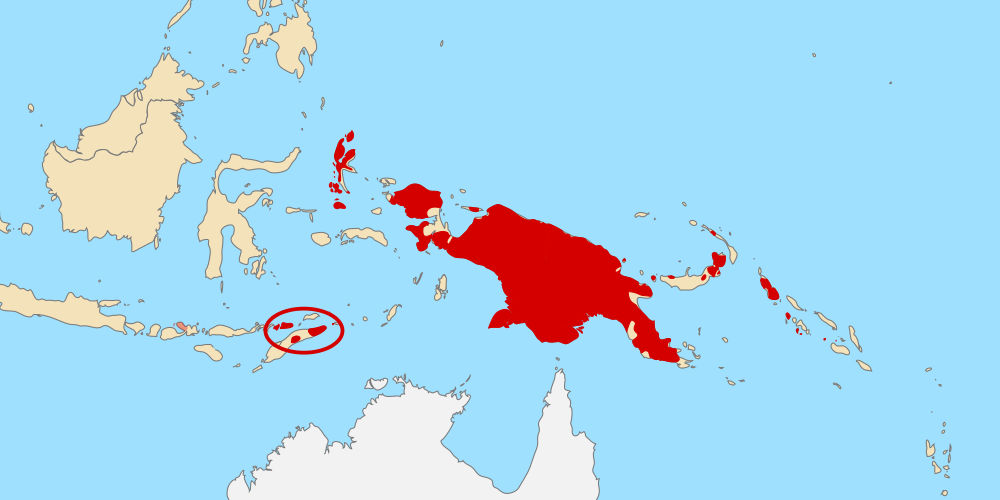
\includegraphics[width=0.8\textwidth]{papuan}\\
  {\footnotesize{Based on Kwamikagami, Wikipedia}}
\end{frame}
\section{Databases}
\begin{frame}{Databases}
  Lexical, grammatical and cultural data

  Lexical data: LexiRumah (\url{https://lexirumah.model-ling.eu})

  \includegraphics[width=\textwidth]{lexirumah}
\end{frame}
\section{Computational Methods}
\section{Results}
\end{frame}
\end{document}

% Local Variables:
% TeX-engine: luatex
% End:
